\documentclass[letterpaper,11pt,oneside,reqno]{article}

%%%%%%%%%%%%%%%%%%%%%%%%%%%%%%%%%%%%%%%%%%%%%%%%%%%%%%%%%%%%

\usepackage[pdftex,backref=page,colorlinks=true,linkcolor=blue,citecolor=red]{hyperref}
\usepackage[alphabetic,nobysame]{amsrefs}

%%%%%%%%%%%%%%%%%%%%%%%%%%%%%%%%%%%%%%%%%%%%%%%%%%%%%%%%%%%%
%main packages
\usepackage{amsmath,amssymb,amsthm,amsfonts,mathtools}
\usepackage{graphicx,color}
\usepackage{upgreek}
\usepackage[mathscr]{euscript}

%equations
\allowdisplaybreaks
\numberwithin{equation}{section}

%tikz
\usepackage{tikz}
\usetikzlibrary{shapes,arrows,positioning,decorations.markings}

%conveniences
\usepackage{array}
\usepackage{adjustbox}
\usepackage{cleveref}
\usepackage{enumerate}
\usepackage{datetime}

%paper geometry
\usepackage[DIV=12]{typearea}

%%%%%%%%%%%%%%%%%%%%%%%%%%%%%%%%%%%%%%%%%%%%%%%%%%%%%%%%%%%%
%draft-specific
\synctex=1
% \usepackage{refcheck,comment}

%%%%%%%%%%%%%%%%%%%%%%%%%%%%%%%%%%%%%%%%%%%%%%%%%%%%%%%%%%%%
%this paper specific
\newcommand{\ssp}{\hspace{1pt}}

%%%%%%%%%%%%%%%%%%%%%%%%%%%%%%%%%%%%%%%%%%%%%%%%%%%%%%%%%%%%
\newtheorem{proposition}{Proposition}[section]
\newtheorem{lemma}[proposition]{Lemma}
\newtheorem{corollary}[proposition]{Corollary}
\newtheorem{theorem}[proposition]{Theorem}
%%%%%%%%%%%%%%%%%%%%%%%%%%%%%%%%%%%%%%%%%%%%%%%%%%%%%%%%%%%%
\theoremstyle{definition}
\newtheorem{definition}[proposition]{Definition}
\newtheorem{remark}[proposition]{Remark}
%%%%%%%%%%%%%%%%%%%%%%%%%%%%%%%%%%%%%%%%%%%%%%%%%%%%%%%%%%%%

\begin{document}
\title{Lectures on Random Matrices
(Spring 2025)
\\Lecture 9: Loop equations and asymptotics to Gaussian Free Field}


\date{Wednesday, March 5, 2025\footnote{\href{https://lpetrov.cc/rmt25/}{\texttt{Course webpage}}
$\bullet$ \href{https://lpetrov.cc/simulations/model/random-matrices/}{\texttt{Live simulations}}
$\bullet$ \href{https://lpetrov.cc/rmt25/rmt25-notes/rmt2025-l09.tex}{\texttt{TeX Source}}
$\bullet$
Updated at \currenttime, \today}}


\author{Leonid Petrov}

\maketitle

\section{Recap}

\subsection{(Dynamical) loop equations}

\begin{theorem}
	\label{Theorem_loop_equation}
 We fix $n=1,2,\dots$ and $n+1$ real numbers $\lambda_1\ge\dots\ge\lambda_{n+1}$. For $\beta>0$, consider $n+1$ i.i.d.\ $\chi^2_\beta$ random variables $\xi_i$ and set
 $$
  w_i=\frac{\xi_i}{\sum_{j=1}^{n+1} \xi_j}, \qquad 1\le i \le n+1.
 $$
 We define $n$ random points $\{\mu_1,\dots,\mu_n\}$ as $n$ solutions to the equation
 \begin{equation} \label{eq_mu_equation}
  \sum_{i=1}^{n+1} \frac{w_i}{z-\lambda_i}=0.
 \end{equation}
 Take any \emph{polynomial} $W(z)$ and consider the complex function:
 \begin{equation}
 \label{eq_loop_observable}
 f_W(z)=\operatorname{\mathbb{E}}\left[\prod_{j=1}^n \exp\bigl(W(\mu_j)\bigr) \frac{\prod_{i=1}^{n+1} (z-\lambda_i)}{\prod_{j=1}^n (z-\mu_j)} \left( W'(z)+\sum_{i=1}^{n+1} \frac{\beta/2-1}{z-\lambda_i} + \sum_{j=1}^n \frac{1}{z-\mu_j}\right)\right].
 \end{equation}
 Then $f_W(z)$ is an \emph{entire function} of $z$, in the following sense:
 \begin{itemize}
	 \item For $z\in \mathbb{C}\setminus [\lambda_{n+1},\lambda_1]$, the expectation in \eqref{eq_loop_observable} defines a holomorphic function of $z$.
  \item This function has an analytic continuation to $\mathbb{C}$, which has no singularities.
 \end{itemize}
\end{theorem}

We proved this statement for $\beta>2$, but it is valid for all $\beta>0$.

\subsection{Loop equations for $W=0$}

When $W=0$, the loop equation \eqref{eq_loop_observable} becomes
\begin{equation*}
	f_0(z)=\frac{(n+1)\beta}{2}-1,
\end{equation*}
so
\begin{equation*}
		\operatorname{\mathbb{E}}\left[\frac{\prod_{i=1}^{n+1}(z-\lambda_i)}{\prod_{j=1}^n(z-\mu_j)}\left(\sum_{i=1}^{n+1}\frac{\beta/2-1}{z-\lambda_i} + \sum_{j=1}^n\frac{1}{z-\mu_j}\right)\right] = \frac{(n+1)\beta}{2}-1.
\end{equation*}

Recall that we defined
\begin{align*}
G_\lambda(z) = \frac{1}{n}\sum_{i=1}^{n+1}\frac{1}{z-\lambda_i},
\qquad
G_\mu(z) = \frac{1}{n}\sum_{j=1}^n\frac{1}{z-\mu_j}.
\end{align*}
We also define the ``logarithmic potentials'' (indefinite integrals of the Stieltjes transforms):
\begin{align*}
\int G_\lambda(z)dz = \frac{1}{n}\sum_{i=1}^{n+1}\ln(z-\lambda_i), \qquad
\int G_\mu(z)dz = \frac{1}{n}\sum_{j=1}^n\ln(z-\mu_j).
\end{align*}
We understand the integrals up to the same integration constant (and branch), so the exponent of the difference
yields the original product:
\begin{equation*}
	\frac{\prod_{i=1}^{n+1}(z-\lambda_i)}{\prod_{j=1}^n(z-\mu_j)} = \exp\left(n\left(\int G_\lambda(z) - \int G_\mu(z)\right)\right)
\end{equation*}
We can rewrite
the loop equation
as:
\begin{equation} \label{eq:stieltjes_transform_eq}
	\operatorname{\mathbb{E}}\left[\exp\left(n\left(\int G_\lambda(z)\,dz - \int G_\mu(z)\,dz\right)\right)\left(\left(\frac{\beta}{2}-1\right)G_\lambda(z) + G_\mu(z)\right)\right] = \frac{\beta}{2} + \frac{1}{n}\left(\frac{\beta}{2}-1\right).
\end{equation}

\subsection{The full corners process}

Assume $n$ is going to infinity, and we fix a sequence of
top-level eigenvalues $\lambda^{(n)}_j$, $1\le j \le n$,
growing in some way. This sequence can be random
(like G$\beta$E rescaled to have eigenvalues in a bounded interval)
or deterministic
(for example, $\lambda^{(n)}$ has $n/10$ points at $0$,
$n/10$ points at $1$, and $8n/10$ points at $2$,
see \Cref{fig:corners}).
\begin{figure}[htpb]
	\centering
	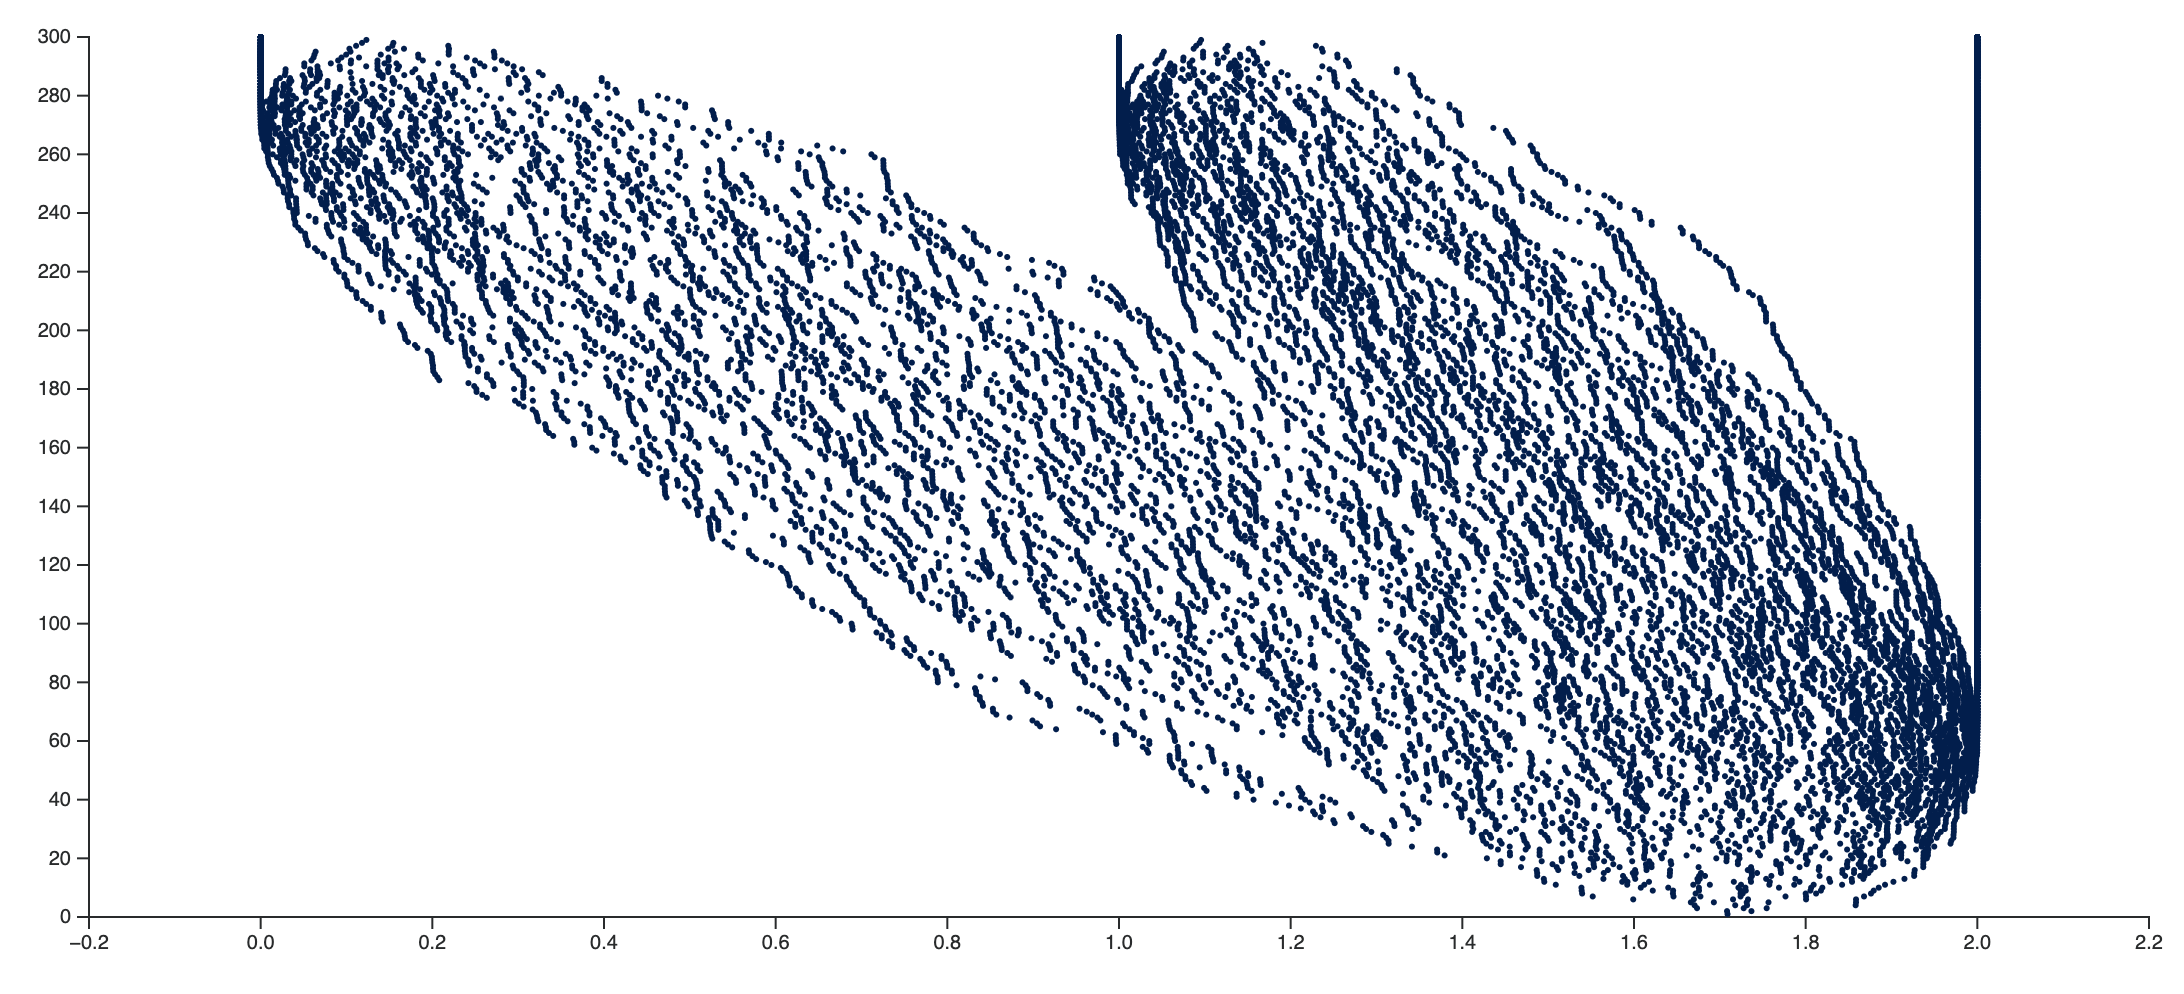
\includegraphics[width=\textwidth]{./pictures/corners.png}
	\caption{Corners process for $n=300$,
	$\beta=1$, with $n/10$ points at $0$,
	$n/10$ points at $1$, and $8n/10$ points at $2$ on the top level.}
	\label{fig:corners}
\end{figure}

Denote the eigenvalues
of the $k\times k$ beta corner (that is,
obtained by successively solving the polynomial equation
\eqref{eq_mu_equation}
$n-k$ times) by $\lambda^{(k)}_j$, $1\le j \le k$.
As $n\to\infty$, we postulate that
\begin{quote}
	The empirical distribution of $\lambda^{(k)}_j$
	converges to some deterministic probability measure
	$\mathfrak{m}_t$, where $k/n\to t\in[0,1]$.
	Consequently, the Stieltjes transform $G_{\lambda^{(k)}}(z)$
	converges to $G_t(z)$, for $z$ in a complex domain
	outside of the support of $\mathfrak{m}_t$.
\end{quote}
Note that we do not assume the scaling of the
$\lambda^{(k)}_j$'s, for convenience.

Denote by $\displaystyle
G_t(z)=\int_{\mathbb{R}}\frac{\mathfrak{m}_t(dx)}{z-x}$
the Stieltjes transform of the measure $\mathfrak{m}_t$.

\begin{proposition}
	The functions $G_t(z)$ satisfy the complex Burgers equation
	\begin{equation*}
		\frac{\partial}{\partial t}G_t(z) +
		\frac{1}{G_t(z)}\frac{\partial}{\partial z}G_t(z) = 0.
	\end{equation*}
\end{proposition}
\begin{proof}
	We have in \eqref{eq:stieltjes_transform_eq},
	if $\lambda$ and $\mu$ live on levels $t$ and $t-\frac{1}{n}$,
	respectively:
	\begin{equation*}
		G_\lambda(z)-G_\mu(z)\approx
		\frac{1}{n}\ssp\frac{\partial}{\partial t}G_t(z),
		\qquad
		\left( \frac{\beta}{2}-1 \right)G_\lambda(z) + G_\mu(z) \approx
		\frac{\beta}{2}\ssp G_t(z) - \frac{1}{n}\ssp\frac{\partial}{\partial t}G_t(z)
		\approx
		\frac{\beta}{2}\ssp G_t(z) .
	\end{equation*}
	Due to the concentration assumption, we can ignore the expectation.
	Then, taking the logarithm of \eqref{eq:stieltjes_transform_eq},
	and differentiating with respect to $z$,
	we get the Burgers equation.
\end{proof}

\subsection{Example: G$\beta$E and the semicircle law}

The Stieltjes transform of the semicircular law is given by:
\begin{equation*}
	G(z) = \int\limits_{-2}^{2}\frac{1}{z-x}\frac{\sqrt{4-x^2}}{2\pi}dx =
	\frac{1}{2} \left(z-\sqrt{z^2-4}\right).
\end{equation*}
We take this as the function $G_t(z)$ for $t=1$.
Then, for each $0\le t\le 1$, the
G$\beta$E solution should be
\begin{equation*}
	\frac{1}{n}\sum_{i=1}^{\lfloor nt \rfloor }\frac{1}{z-\lambda_i^{(\lfloor nt \rfloor )}}
	\to t\ssp G^{(\sqrt t)}(z),
\end{equation*}
where
\begin{equation*}
	G^{(c)}(z) \coloneqq \frac{z-\sqrt{z^2-4c^2}}{2c^2},
\end{equation*}
is the Stieltjes transform of the semicircular law on $[-2c, 2c]$.

\begin{lemma}
	\label{lemma:semicircle_and_burgers}
	The function $G_t(z)\coloneqq t\ssp G^{(\sqrt t)}(z)$
	satisfies the Burgers equation.
\end{lemma}
\begin{proof}
	Straightforward verification.
\end{proof}



\section{Gaussian Free Field}
\label{sec:GFF}

The \emph{Gaussian Free Field} (GFF) is a fundamental object in probability theory and mathematical physics. Roughly speaking, it can be viewed as a multi-dimensional analog of Brownian motion: instead of one-dimensional “time,” the underlying parameter space is a multi-dimensional domain (often two-dimensional). In one dimension, the GFF reduces to an ordinary Brownian bridge (or motion). In higher dimensions, it becomes a random generalized function (a “distribution”) whose covariance structure is governed by the appropriate Green's function of the Laplacian. Below we provide an introduction, starting from finite-dimensional Gaussian vectors and culminating in the GFF as a random distribution.

\subsection{Gaussian correlated vectors and random fields}
\label{subsec:gauss_vectors_random_fields}

Recall that an $n$-dimensional real-valued random vector $X = (X_1,\dots, X_n)$ is called \emph{Gaussian} if every linear combination
\[
\alpha_1 X_1 + \cdots + \alpha_n X_n
\]
of its components is a univariate Gaussian random variable. The law of such a vector is completely determined by its mean vector $m \in \mathbb{R}^n$ and its covariance matrix $\Sigma \in \mathbb{R}^{n\times n}$. The density function, for invertible $\Sigma$, is
\[
f_{X}(x) \;=\; \frac{1}{\sqrt{(2\pi)^n \det \Sigma}}
\exp\Bigl(-\tfrac{1}{2}\,(x - m)^\top \Sigma^{-1}(x - m)\Bigr).
\]
For simplicity, we will assume that $m = 0$ (the centered case).

\subsection{Gaussian fields as random generalized functions}

A natural extension from finite-dimensional Gaussian vectors to infinite-dimensional settings leads us to Gaussian fields. Informally, a Gaussian field is a collection of Gaussian random variables indexed by points in some space.

For a domain $D \subset \mathbb{R}^d$, we might wish to
define a random function $\Phi: D \rightarrow \mathbb{R}$
such that for any finite collection of points $x_1, \ldots,
x_n \in q$, the vector $(\Phi(x_1), \ldots, \Phi(x_n))$ is a
Gaussian vector. However, such a random function may not
exist as a proper function in the usual sense.
The reason is that we would like to consider analogues of linear combinations
of the form
\begin{equation}
	\label{eq:Phi_test_function}
    \Phi(f) = \int_D \Phi(x) f(x) \, dx,
\end{equation}
For example, if we wish the vector $(\Phi(x_1), \ldots, \Phi(x_n))$ to have independent components, we would need to assign a value to each point in $D$. This means that the hypothetical function $\Phi$ would be too irregular, and even non-measurable, and the integral
\eqref{eq:Phi_test_function} would not be well-defined.

Instead, for the field with independent values at all points, we would like $\Phi(f)$ to be normal
with mean zero and variance (paralleling the finite-dimensional story)
\begin{equation*}
	\operatorname{\mathrm{Var}}\left(
	\Phi(f)\right) = \|f\|^2_{L^2(D)} \;=\; \int_D f(x)^2 \, dx.
\end{equation*}
So, Gaussian fields (in particular, our topic, the \emph{Gaussian Free Field})a
are defined as random distributions, not as functions.
That is, rather than assigning a value to each point,
we assign a random value to each test function $f$ in some appropriate space
via \eqref{eq:Phi_test_function}.

The covariance structure of the mean zero Gaussian random variables
$\Phi(f_1), \ldots, \Phi(f_n)$ is given by a certain bilinear
form determined by the domain $D$.


\subsection{Concrete treatment via orthogonal functions}

Let us now construct the Gaussian Free Field more concretely. Consider a bounded domain $D \subset \mathbb{R}^d$ with smooth boundary. Let $\{f_n\}_{n=1}^{\infty}$ be an orthonormal basis of $L^2(D)$ consisting of eigenfunctions of the Laplacian with Dirichlet boundary conditions:
\begin{equation}
    \begin{cases}
        -\Delta f_n = \lambda_n f_n & \text{in } D, \\
        f_n = 0 & \text{on } \partial D,
    \end{cases}
\end{equation}
where $0 < \lambda_1 \leq \lambda_2 \leq \ldots$ are the corresponding eigenvalues.

We can now define the Gaussian Free Field on $D$ as:
\begin{equation}
    \Phi = \sum_{n=1}^{\infty} \frac{\alpha_n}{\sqrt{\lambda_n}} f_n,
\end{equation}
where $\{\alpha_n\}_{n=1}^{\infty}$ are independent standard Gaussian random variables. This series does not converge pointwise, but it does converge in the space of distributions almost surely.

For any test function $g \in C_0^{\infty}(D)$, we have:
\begin{equation}
    \Phi(g) = \int_D \Phi(x) g(x) \, dx = \sum_{n=1}^{\infty} \frac{\alpha_n}{\sqrt{\lambda_n}} \int_D f_n(x) g(x) \, dx,
\end{equation}
which is a well-defined Gaussian random variable.

\subsection{Connection to Brownian bridge}

The Gaussian Free Field in one dimension is closely related to the Brownian bridge. Consider the interval $[0,1]$ with the Dirichlet Laplacian. The eigenfunctions are $f_n(x) = \sqrt{2} \sin(n\pi x)$ with eigenvalues $\lambda_n = n^2 \pi^2$. The Gaussian Free Field on $[0,1]$ can be expressed as:
\begin{equation}
	\label{eq:Phi_1d}
    \Phi(x) = \sqrt{2} \sum_{n=1}^{\infty} \frac{\alpha_n}{n\pi} \sin(n\pi x).
\end{equation}
This series representation converges to a continuous function, which is precisely the Brownian bridge on $[0,1]$. The Brownian bridge is a Gaussian process $B_t$ with mean zero and covariance function:
\begin{equation}
	\label{eq:covariance_1d}
    \mathbb{E}[B_s B_t] = \min(s, t) - st.
\end{equation}
The key difference between the one-dimensional and higher-dimensional cases is that in one dimension, the Gaussian Free Field is a continuous function, whereas in dimensions two and higher, it is a genuine distribution (not a function). This reflects the fact that Brownian motion is a continuous path in one dimension but becomes increasingly irregular in higher dimensions.

\subsection{Covariance structure and Green's function}

The covariance structure of the Gaussian Free Field is intimately connected to the Green's function of the Laplacian. For test functions $f, g \in C_0^{\infty}(D)$, we have:
\begin{align}
    \mathbb{E}[\Phi(f) \Phi(g)] &= \mathbb{E}\left[\sum_{n,m=1}^{\infty} \frac{\alpha_n \alpha_m}{\sqrt{\lambda_n \lambda_m}} \int_D f_n(x) f(x) \, dx \int_D f_m(y) g(y) \, dy\right] \\
    &= \sum_{n=1}^{\infty} \frac{1}{\lambda_n} \int_D f_n(x) f(x) \, dx \int_D f_n(y) g(y) \, dy.
\end{align}
Define the Green's function $G_D(x, y)$ for the Dirichlet Laplacian on $D$ as the solution to:
\begin{equation}
    \begin{cases}
        -\Delta_x G_D(x, y) = \delta(x - y) & \text{for } x, y \in D, \\
        G_D(x, y) = 0 & \text{for } x \in \partial D \text{ or } y \in \partial D.
    \end{cases}
\end{equation}
The Green's function has the eigenfunction expansion:
\begin{equation}
    G_D(x, y) = \sum_{n=1}^{\infty} \frac{f_n(x) f_n(y)}{\lambda_n}.
\end{equation}
Using this, we can rewrite the covariance as:
\begin{equation}
	\operatorname{\mathbb{E}}[\Phi(f) \Phi(g)] = \int_D \int_D G_D(x, y) f(x) g(y) \, dx \, dy.
\end{equation}
This relationship between the covariance of the GFF and the Green's function is fundamental. It shows that the GFF can be viewed as a random solution to the equation $-\Delta \Phi = W$, where $W$ is white noise.
Here the white noise is the Gaussian
field with covariance $\delta(x-y)$ --- the object which is the
correct way of constructing a Gaussian field with i.i.d.
values at all points.

\subsection{The GFF on the upper half-plane}

In the complex upper half-plane
$\left\{ \operatorname{Im}z>0 \right\}$
with $\mathbb{R}$ as the boundary,
the Green function has the form
\begin{equation*}
	G(z,w) = -\frac{1}{\pi}\ln|z-w| + \frac{1}{\pi}\ln|z-\overline{w}|.
\end{equation*}
The covariance is
\begin{equation*}
	\operatorname{\mathbb{E}}
	\left[ \Phi(f)\ssp \Phi(g) \right]=
	\int\int|dz|^2\ssp |dw|^2
	f(z)g(w) G(z,w) .
\end{equation*}

\section{Fluctuations}

\subsection{Height function and related definitions}

Let us define the \emph{height function} using the corners process
$\{ \lambda^{(k)}_j\colon 1\le j\le k\le n \}$:
\begin{equation*}
	h(t,x)\coloneqq \#
	\{ \textnormal{eigenvalues $\lambda^{(\lfloor nt \rfloor )}_j$ which
	are $\leq x$} \}.
\end{equation*}
Recall that in our regime, we do not scale $x$.
Throughout the following, we will interchangeably use
the parameters $n$ and
$\varepsilon\coloneqq 1/n$.

Our goal is to understand the asymptotic behavior of the centered height function
$$
h(\varepsilon^{-1}t, x) - \mathbb{E}[h(\varepsilon^{-1}t, x)]
,
$$
defined inside the region of the $(t,x)$ plane.
Note that in contrast with the usual Central Limit Theorem,
the fluctuations are not scaled by $\varepsilon^{1/2}$,
but rather are unscaled.
Note that the law of large numbers is going to be
\begin{equation*}
	\varepsilon
	\ssp h(\varepsilon^{-1}t, x) \to
	\mathfrak{h}(t,x),
\end{equation*}
where $\mathfrak{h}(t,x)$ is the limiting height function
(for a fixed $t$, this is the cumulative distribution function
of the measure $\mathfrak{m}_t$).
We will see that these unscaled fluctuations are
converging to a Gaussian Free Field. Thus,
the unscaled fluctuations
are ``just barely'' going to infinity,
while retaining nontrivial and bounded correlations.

Define
\begin{equation}
	\label{eq:rho_definition}
	\rho(t,x) \coloneqq h(t,x-\varepsilon)-h(t,x)= \sum_{i=1}^{\lfloor nt \rfloor }
	\mathbf{1}_{\lambda_i^{(\lfloor nt \rfloor )}\le x\le \lambda_{i}^{(\lfloor nt \rfloor )}+\varepsilon},\qquad \textnormal{where $\mathbf{1}_A$ is the indicator of the event $A$.}
\end{equation}
This is a discrete analogue of the $x$-derivative of $h(t,x)$.

% Let the support of $\mathfrak{m}_t$ be compact, $[l(t),r(t)]$.
% The pre-limit centered Stieltjes transform is
% \begin{equation*}
%   \overline G_t(z)\coloneqq \int_{l(t)}^{r(t)}\frac{\rho(t,x)}{z-x}dx-
%   \operatorname{\mathbb{E}}\left[
%   \int_{l(t)}^{r(t)}\frac{\rho(t,x)}{z-x}dx
%   \right],\qquad z\in \mathbb{C}\setminus [l(t),r(t)].
% \end{equation*}

% \subsection{Main result \cite[Section~6]{gorin2022dynamical}}
%
% As $\varepsilon\to0$, we have
% \begin{equation*}
%   \frac{\overline G_{t+\varepsilon}(z)-\overline G_t(\varepsilon)}{\varepsilon}
%   =
%   \frac{\partial}{\partial z}\left[
%     \overline
%     G_t(z)\frac{\operatorname{\mathbb{E}}\tilde f_t(z)}{1-\operatorname{\mathbb{E}}\tilde f_t(z)}
%   \right]+
%   \Delta M_t(z)+R,
% \end{equation*}
% where the remainder is small, and $\Delta M_t(z)$ are mean zero,
% and $\varepsilon^{-1/2}\Delta M_t(z)$ are asymptotically Gaussian with the limiting covariance
% \begin{equation*}
%   \frac{\operatorname{\mathbb{E}}\left[ \Delta M_t(z_1)\Delta M_{t'}(z_2) \right]}{\varepsilon}
%   =
%   \frac{\delta_{t=t'}}{2\pi i}\oint
%   \frac{f_t(w)}{f_t(w)-1}
%   \frac{1}{(w-z_1)^2(w-z_2)^2}\ssp dw+o(1).
% \end{equation*}
% In other words, we have lots of Gaussian observables, and this hints at the Gaussian Free Field
% limit.
%
% Here $f_t,\tilde f_t$ are certain functions constructed explicitly from the model, to be seen later.
%
\subsection{Key theorem on the way to the main result}

This subsection recreates the argument analogous to 
\cite[Theorem~4.5]{gorin2022dynamical},
but in the random matrix setting.

This theorem is an asymptotic expansion of the Stieltjes transform
of the one-step transition from $\lambda$ to $\mu$.
We assume that the support of $\lambda$ is in $[l,r]$.
Denote 
\begin{equation*}
	\Pi_\lambda(z)\coloneqq \prod_{i=1}^{n+1}(z-\lambda_i),\qquad 
	\Pi_\mu(z)\coloneqq \prod_{j=1}^{n}(z-\mu_j).
\end{equation*}
Also assume that $W(z)$ is fixed and nice, and that $\mu_j$ are 
distributed according to a modified 
density, which includes $W(z)$:
\begin{equation*}
	\frac{1}{Z}
		\prod_{1\le i<j\le n}(\mu_i-\mu_j)
		\prod_{i=1}^{n}\prod_{j=1}^{n+1} |\mu_i-\lambda_j|^{\beta/2-1}
		\prod_{1\le i<j\le n+1}(\lambda_i-\lambda_j)^{1-\beta}\prod_{j=1}^n e^{W(\mu_j)}.
\end{equation*}
From now on, all expectations will be over the modified density.

We aim to analyze the quantity
\begin{equation*}
	\mathcal{A}(z)\coloneqq\operatorname{\mathbb{E}}\left[ \frac{\Pi_\lambda(z)}{\Pi_\mu(z)} \right],
\end{equation*}
which enters the loop equation. Moreover, the loop equation
states the holomorphicity of
\begin{equation*}
	\mathcal{C}(z)=
	\mathcal{A}(z)\Biggl[ W'(z)+ \frac{\beta}{2}\frac{1}{n}\sum_{i=1}^{n+1}\frac{1}{z-\lambda_i} \Biggr]+
	\operatorname{\mathbb{E}}
	\Biggl[ 
		\frac{\Pi_\lambda(z)}{\Pi_\mu(z)}\Biggl(\frac{1}{n}\sum_{j=1}^{n}\frac{1}{z-\mu_j}-
		\frac{1}{n}\sum_{i=1}^{n+1}\frac{1}{z-\lambda_i}\Biggr)
	\Biggr].
\end{equation*}
It will turn out that the first summand is the leading term, and the second summand will be 
negligible.



\newpage
\colorbox{yellow}{\parbox{.7\textwidth}{rewrite}}

Let $\rho_\mu(x)$ stand for \eqref{eq:rho_definition} with $\mu$ instead of $\lambda^{(\lfloor nt \rfloor )}$. Define
\begin{equation*}
	\mathcal{G}_\mu(z)=\exp\left[ \int_{l}^{r} \frac{\rho_\mu(x)}{z-x}\ssp dx\right],
	\qquad 
	\mathcal{B}_\mu(z)=1+\mathcal{G}_\mu(z)\colorbox{yellow}{\parbox{.7\textwidth}{loop eq}}
\end{equation*}
We have
\begin{equation*}
	\int_l^r\frac{\rho_\mu(x)}{z-x}dx=\sum_{i=1}^n
	\sum_{i=1}^n\int_{\mu_i}^{\mu_i+\varepsilon}\frac{dx}{z-x}=
	\sum_{i=1}^n\left( \ln(z-\mu_i+\varepsilon)-\ln(z-\mu_i) \right), 
\end{equation*}
so
\begin{equation*}
	\mathcal{G}_\mu(z)=\prod_{i=1}^{n}\frac{z-\mu_i+\varepsilon}{z-\mu_i}=
	1+\varepsilon\sum_{i=1}^{n}\frac{1}{z-\mu_i}+O(\varepsilon^2)..
\end{equation*}

\begin{theorem}
	We have as $\varepsilon\to0$:
	\begin{equation*}
		\frac{1}{\varepsilon}\int_l^r \frac{\rho_\mu(x)-\rho_\lambda(x)}{z-x}\ssp dx
		=
		\frac{1}{\pi i \beta}\oint_{\omega_-} \frac{\ln \mathcal{B}_\mu(z)}{(w-z)^2}\ssp dw
		+
		\varepsilon\cdot\left( \textnormal{explicit expression} \right)
		+\Delta M(z)+O(\varepsilon^2),
	\end{equation*}
	where the contour $\omega_-$ encloses $[l,r]$ but not $z$,
	and $\Delta M(z)$ are mean $0$ random variables such that $\varepsilon^{-1/2}\Delta M(z)$,
	for $z\mathbb{C}\setminus [l,r]$, are asymptotically Gaussian with the limiting covariance
	\begin{equation*}
		\frac{\operatorname{\mathbb{E}}\left[ 
		\Delta M(z_1)\Delta M(z_2) \right]}{\varepsilon}
			=
		\frac{1}{\pi i \beta}\oint_{\omega_-}
		\frac{\mathcal{G}(w)\varphi^+(w)}{\mathcal{B}(w)}\frac{dw}{(w-z_1)^2(w-z_2)^2}+o(1).
	\end{equation*}
	The higher order joint moments of $\varepsilon^{-1/2}\Delta M(z)$ 
	also converge as $\varepsilon\to0$ to Gaussian moments.
\end{theorem}



\appendix
\setcounter{section}{8}

\section{Problems (due 2025-04-29)}

\subsection{Brownian bridge}

Derive the covariance structure of the Brownian bridge
\eqref{eq:covariance_1d} from the series representation
\eqref{eq:Phi_1d}.



\bibliographystyle{alpha}
\bibliography{bib}


\medskip

\textsc{L. Petrov, University of Virginia, Department of Mathematics, 141 Cabell Drive, Kerchof Hall, P.O. Box 400137, Charlottesville, VA 22904, USA}

E-mail: \texttt{lenia.petrov@gmail.com}


\end{document}
